% This is "sig-alternate.tex" V2.0 May 2012
% This file should be compiled with V2.5 of "sig-alternate.cls" May 2012
%
% For tracking purposes - this is V2.0 - May 2012

\documentclass{sig-alternate}
\usepackage{graphicx}
\usepackage{subfigure}
\usepackage{url}
\usepackage{indentfirst}
\usepackage{cite}


\usepackage{color}
\newcommand{\red}[1]{\textcolor{red}{#1}}
\newcommand{\blue}[1]{\textcolor{blue}{#1}}



\usepackage[normalem]{ulem}


\begin{document}
%
% --- Author Metadata here ---
\conferenceinfo{MSND}{'13 Rio de Janeiro, Brazil}
%\CopyrightYear{2007} % Allows default copyright year (20XX) to be over-ridden - IF NEED BE.
%\crdata{0-12345-67-8/90/01}  % Allows default copyright data (0-89791-88-6/97/05) to be over-ridden - IF NEED BE.
% --- End of Author Metadata ---

\title{Temporal Evolution of Scientific Communities}
%\title{The Role of Leaders in the Dynamics of Scientific Communities}


\numberofauthors{3} %  in this sample file, there are a *total*
\author{
%
% 1st. author
\alignauthor Bruno Leite Alves\\
       \affaddr{UFMG}\\
       \affaddr{Belo Horizonte, Brazil}\\
       \email{bruno.leite@dcc.ufmg.br}
% 2nd. author
\alignauthor Fabr\'icio Benevenuto\\
       \affaddr{UFMG}\\
       \affaddr{Belo Horizonte, Brazil}\\
       \email{fabricio@dcc.ufmg.br}
% 3rd. author
\alignauthor Alberto H. F. Laender\\
      \affaddr{UFMG}\\
      \affaddr{Belo Horizonte, Brazil}\\
      \email{laender@dcc.ufmg.br}
}

\maketitle
\begin{abstract}

\end{abstract}

% A category with the (minimum) three required fields
\category{H.4}{Social Network}{Temporal Analisys}
%A category including the fourth, optional field follows...
%\category{D.2.8}{Software Engineering}{Metrics}[complexity measures, performance measures]
\category{J.4.} {Computer Applications} Social and behavioral sciences {Miscellaneous}

\terms{Human Factors, Measurement.}


\keywords{communities, scientific communities, core community, evolution}

\section{Introduction}

Since its beginning, society has been organizing itself into communities, which are groups of people with common interests. Particularly, the proliferation of new communication
technologies based on the Internet has facilitated the rapid formation and growth of online communities. Communities exhibit a wide range of characteristics and serve a variety of
purposes, from small groups engaged in tightly niche topics such as a very specific scientific community, to millions of users linked by an interest such as a community related to
a sport team or fans of a celebrity. 

Often, individuals who are socially connected in a community tend to share interests and similarities. Although, there are many factors that might determine a community formation
and its growth, there are two main driven forces used to explain similarity in a community formation: influence and homophily. On one hand, influence posits that individuals change
to become more similar to their friends in the community. On the other hand, homophily postulates that individuals create social connections within a community precisely because
they are already similar. Recent efforts have provided quantitative evidences of both forces~\cite{icwsm10cha,crandall.kdd08,Backstrom:2006,influence.correlation.kdd08} and
existing theories~\cite{Rogers.1962,accidental-influential}, models~\cite{kempe03kdd,Kempe05influentialnodes}, and
approaches~\cite{saez-trumper@kdd12,Weng:2010:TFT:1718487.1718520} rely on identifying a group of influential individuals with the power to affect not only the underlying network
structure of a community, but also to interfere on the spread and flow of information within a community. 

In this paper, we take a different perspective and study a complementary problem. Here, we focus on studying the roles that scientific community leaders play and how they can impact intrinsic
evolving properties of research communities. When prolific research leaders decide to join or leave communities, they take with them resources,
experience, students and they possibly influence other authors to do the same, which makes scientific communities very suitable for this kind of study. We used data from DBLP to identify
scientific communities, represented by the main ACM SIGs conferences. Then, we propose a strategy to infer the community core, the leaders of a given scientific community in a
given period of time. Finally, we investigate how aspects of the core impact on the community structure. 

The study of the community core of scientific communities is of interest from two different perspectives.  The first is sociological, steemming from the necessity to understand how
segments of society evolve as well as to answer longstanding  questions related to the interaction among different types of participants. On the other hand, from a technological perspective,
understanding  these aspects is critical not only for link prediction as well as the designing better recommendation systems, but it is also a necessary step for viral marketing
strategies and social campaigns.  Such a study, however, has been difficult as essential components like human connections and a proper definition of leadership is hard to be
reproduced at a large scale within the confines of a research laboratory.

Our results show that (\red{TO DO}). 


The rest of this paper is organized as follows. Next section surveys related efforts. Then, Section 3 describes our strategy and dataset used to construct the connections around
scientific communities and analyzes the main evolving properties of this communities.  Section 4 describes our strategy to compute the community core and Section 5 investigate the
main properties of these sets of authors within their communities.  Finally, Section 6 concludes the paper and provides directions for future work. 





\section{Related Work}


There has been a number of recent efforts that attempt to analyze community structure and network evolution.  Particularly, Kumar \textit{et al.}~\cite{Kumar:2006} analyzed two large networks to
find a segmentation of these networks into singletons, isolated communities, a giant component. Then, they propose a network growth model able to generate networks with similar
characteristics.  Ducheneaut \textit{et al.}~\cite{Ducheneaut:2007} extracted and characterized explicitly created communities from the World of Warcraft, a massive multiplayer game.
Complementarily, Patil \textit{et al.}~\cite{Patil:2012} analyzed and modeled factors that make users to leave or join on-line gaming communities.  Viswanath \textit{et
al.}~\cite{Viswanath:2009} studied the evolution of activity between users in Facebook and found that that links in the activity network tend to come and go rapidly over time, and
the strength of ties exhibits a general decreasing trend of activity as the social network link ages.

In terms of models for network dynamics, Leskovec \textit{et al.}~\cite{Leskovec:2005} investigated a wide range of real graphs to show that graphs densify over time, with the
number of edges growing super linearly in the number of nodes and that the average distance between nodes often shrinks over time. Based on these observations, they develop a graph
generation model that incorporates such properties.  More recently, Leskovec \textit{et al.}~\cite{Leskovec:2008} presented a detailed study of network evolution by analyzing four
large on-line social networks.  They investigated a wide variety of network formation strategies to show that edge locality plays a critical role in the evolution of networks. Based on
this observation, they developed a model of network evolution, in which nodes arrive at a pre-specified rate.  Differently from the above efforts, our work focuses on community
properties and the roles that community leaders play in the underlying network structure.

There are also efforts that attempted to study scientific communities. Particularly, Backstrom \textit{et al.}\cite{Backstrom:2006} studied communities in LiveJournal and
scientific communities extracted from DBLP to find that the propensity of individuals to join communities and of communities to grow rapidly, depends in subtle ways on the
underlying network structure. Huang \textit{et al.}~\cite{Huang:2008} used DBLP data to construct a network for the Computer Science field covering research collaborations from
1980 to 2005. Among their main observations, they show that the Computer Science field presents a collaboration pattern more similar to Mathematics than to Biology.  
Different from these efforts, here we focus on studying the properties of the community core, thus our analyses are complementary to
theirs.

Finally, when it comes to identifying the community core, there are many approaches that extract the core based on structural properties of the underlying
network~\cite{Leskovec@www2010,Chakrabarti:2006:EC:1150402.1150467,citeulike:370723,Sachan:2012}.  Particular, 
Seifi \textit{et al.}~\cite{Seifi:2012:CCE:2187980.2188258} combined four different
approaches to identify a community core and characterized some properties of the obtained cores. Such approach is not applicable to our context, as we are interested in studying
network properties of the community core. 



\section{Scientific Communities}


The notion of community can be understood as a dense group of nodes in a network, with more edges inside than edges linking the rest of the network.  There are multiple definitions
and strategies of identifying communities and they vary according to the context. In our context, a scientific community is defined in terms of a large and well established
scientific conference able to aggregate authors working in similar research topics along a considerable number of years. Next, we describe how we have built a large set of
scientific communities.


In order to build a set of scientific communities to study, we have gathered data from DBLP\footnote{http://dblp.uni-trier.de/}~\cite{Ley:2009}, a digital library containing more
than 2.1 million publications from 1.2 million authors that provides bibliographic information on major Computer Science conference proceedings and journals.  DBLP offers its
entire database in XML format, which facilitates gathering and reconstructing entire scientific communities. 

Each publication is accompanied by its title, list of authors, year of publication, and publication venue, i.e., the conference or journal. For the purposes of our work, we
consider a scientific community as a graph in which nodes represent researchers and edges links coauthors of papers from the same community.  In order to define such communities,
we focus on the publications from the flagship conferences of major ACM SIGs (Special Interest Groups).  Thus, we define a scientific community by linking people that have
coauthored a paper in a certain conference, making the flagship conferences of the ACM SIGs to act as communities where coauthorships are formed. We have removed young conferences
without enough data for a temporal analysis as well as conferences whose entire history is not registered on DBLP, to allow us carrying out temporal analyses. In total, 24
scientific communities were considered. Table~\ref{tab:sigs_conference_period} lists these communities, including the respective ACM SIG, the conference acronym, the period
considered (some conferences had the period reduced to avoid hiatus in the data), the h-index\footnote{Obtained from the SHINE (Simple H-INdex Estimator) projet:
http://shine.icomp.ufam.br.} and the total number of authors, publications and editions as well as ratios extracted from these last three figures.

\begin{table*}[!htb]
\centering
\caption{The data of DBLP of flagship conferences of ACM SIGs}
\label{tab:sigs_conference_period}
{\small
\begin{tabular}{|l|l|c|c|c|c|c|c|c|c|} \hline
SIG & Conference & Period & H-Index & Authors & Publications & Editions & Aut/Edi & Pub/Edi & Aut/Pub\\ \hline
SIGACT & STOC & 1969-2012 & 94 & 2159 & 2685 & 44 & 49.07 & 61.02 & 0.80\\ \hline
SIGAPP & SAC & 1993-2011 & 59 & 9146 & 4500 & 19 & 481.37 & 236.84 & 2.03\\ \hline
SIGARCH & ISCA & 1976-2011 & 102 & 2461 & 1352 & 36 & 68.36 & 37.56 & 1.82\\ \hline
SIGBED & HSCC & 1998-2012 & - & 846 & 617 & 15 & 56.40 & 41.13 & 1.37\\ \hline
SIGCHI & CHI & 1994-2012 & 144 & 5095 & 2819 & 19 & 268.16 & 148.37 & 1.81\\ \hline
SIGCOMM & SIGCOMM & 1988-2011 & 140 & 1593 & 796 & 24 & 66.38 & 33.17 & 2.00\\ \hline
SIGCSE & SIGCSE & 1986-2012 & 51 & 3923 & 2801 & 27 & 145.30 & 103.74 & 1.40\\ \hline
SIGDA & DAC & 1964-2011 & 98 & 8876 & 5693 & 48 & 184.92 & 118.60 & 1.56\\ \hline
SIGDOC & SIGDOC & 1989-2010 & 23 & 1071 & 810 & 22 & 48.68 & 36.82 & 1.32\\ \hline
SIGGRAPH & SIGGRAPH & 1985-2003 & 119 & 1920 & 1108 & 19 & 101.05 & 58.32 & 1.73\\ \hline
SIGIR & SIGIR & 1978-2011 & 116 & 3624 & 2687 & 34 & 106.59 & 79.03 & 1.35\\ \hline
SIGKDD & KDD & 1995-2011 & 124 & 3078 & 1699 & 17 & 181.06 & 99.94 & 1.81\\ \hline
SIGMETRICS & SIGMETRICS & 1981-2011 & 71 & 2083 & 1174 & 31 & 67.19 & 37.87 & 1.77\\ \hline
SIGMICRO & MICRO & 1987-2011 & 81 & 1557 & 855 & 25 & 62.28 & 34.20 & 1.82\\ \hline
SIGMM & Multimedia & 1993-2011 & 80 & 5400 & 2928 & 19 & 284.21 & 154.11 & 1.84\\ \hline
SIGMOBILE & MobiCom & 1995-2011 & 106 & 1151 & 480 & 17 & 67.71 & 28.24 & 2.40\\ \hline
SIGMOD & SIGMOD & 1975-2012 & 147 & 4202 & 2669 & 38 & 110.58 & 70.24 & 1.57\\ \hline
SIGOPS & PODC & 1982-2011 & 59 & 1685 & 1403 & 30 & 56.17 & 46.77 & 1.20\\ \hline
SIGPLAN & POPL & 1975-2012 & 85 & 1527 & 1217 & 38 & 40.18 & 32.03 & 1.25\\ \hline
SIGSAC & CCS & 1996-2011 & 97 & 1354 & 676 & 16 & 84.63 & 42.25 & 2.00\\ \hline
SIGSAM & ISSAC & 1988-2011 & - & 1100 & 1177 & 24 & 45.83 & 49.04 & 0.93\\ \hline
SIGSOFT & ICSE & 1987-2011 & 111 & 3502 & 2248 & 25 & 140.08 & 89.92 & 1.56\\ \hline
SIGUCCS & SIGUCCS & 1989-2011 & - & 1771 & 1593 & 23 & 77.00 & 69.26 & 1.11\\ \hline
SIGWEB & CIKM & 1992-2011 & 82 & 4978 & 2623 & 20 & 248.90 & 131.15 & 1.90\\ \hline
\end{tabular}
}
\end{table*}





%\begin{figure*}
%\centering
%\includegraphics[scale=.4]{graficos/sigs_metricas_acumuladas_1_em_1_ano/assortatividade_grupo_temporal_web.eps}
%\caption{Assortativity accumulated from 1 in 1 year}
%\label{fig:assortativity_1_in_1}
%\end{figure*}

%\begin{figure*}
%\centering
%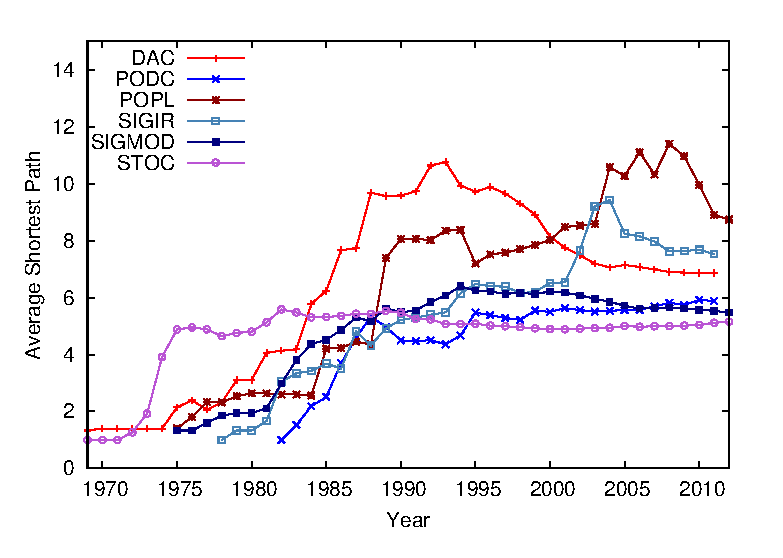
\includegraphics[scale=.4]{graficos/sigs_metricas_acumuladas_1_em_1_ano/caminho_minimo_medio_grupo_temporal_web.eps}
%\caption{Average shortest path accumulated from 1 in 1 year}
%\label{fig:average_shortest_path_1_in_1}
%\end{figure*}

%\begin{figure*}
%\centering
%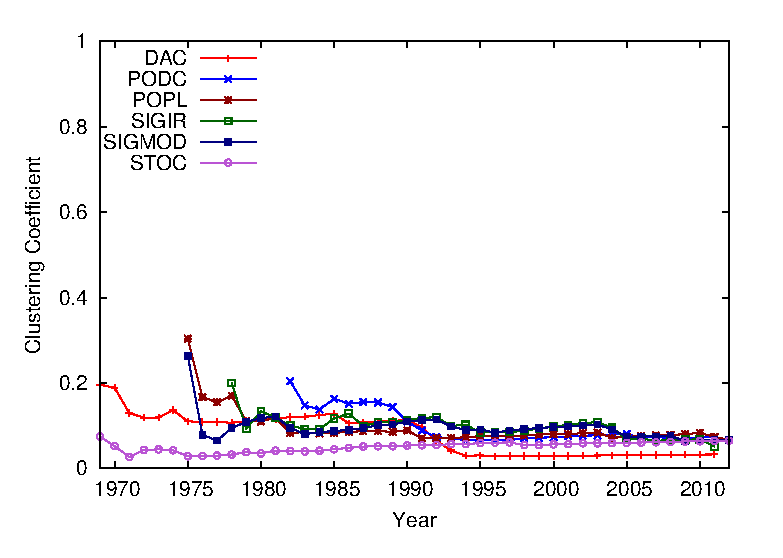
\includegraphics[scale=.4]{graficos/sigs_metricas_acumuladas_1_em_1_ano/coeficiente_agrupamento_grupo_temporal_web.eps}
%\caption{Clustering Coefficient accumulated from 1 in 1 year}
%\label{fig:clustering_coefficient_1_in_1}
%\end{figure*}

%\begin{figure*}
%\centering
%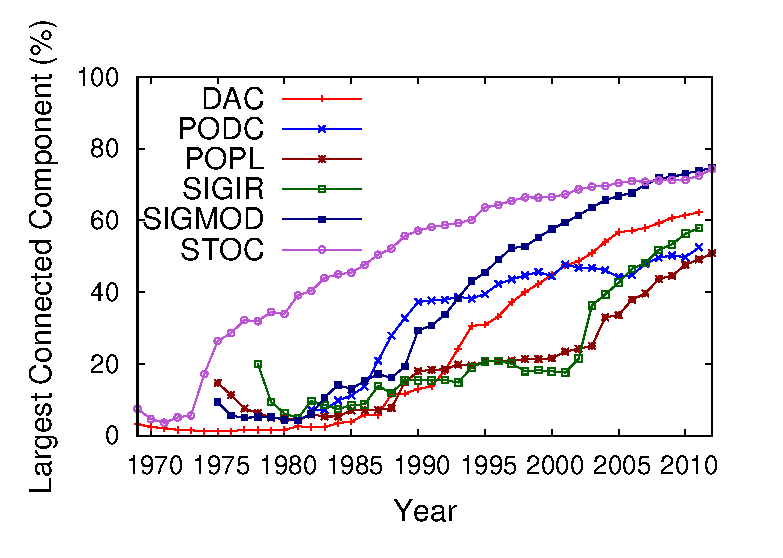
\includegraphics[scale=.4]{graficos/sigs_metricas_acumuladas_1_em_1_ano/porcentagem_maior_componente_grupo_temporal_web.eps}
%\caption{Largest connected component accumulated from 1 in 1 year}
%\label{fig:largest_connected_component_1_in_1}
%\end{figure*}




\input{core.tex}
\section{Properties of the communities core}

In this section we explain about the main properties of the what we define as core communities in the previous sections.
We also show how the core community behaves in some social networks metrics and how its impacts yours communities over 
the years using temporal slide windows.

\subsection{Core over time}
Thus as the communities, the core community also evolves over the years. The Figure \ref{fig:metrics_accumulated_1_in_1}
showns how the communities evolves over the time considering data accumulated. Here, we show a different way to see the evolution,
the Figure \ref{fig:metrics_slide_window} showns the evolution of the communities over the year over the years using temporal slide 
window. It is possible to clearly see some differences, as the assortativity in Figure \ref{fig:assortativity_1_in_1}
and Figure \ref{fig:assortativity_slide_window} which in the first one, it start at 1 in many cases and stabilizes at 0 
nowadays, however, the slide windows show a large variation over the time, this may indicate, peharps, that the community come by
more variation than expected. This vision is so important to understand the core community, how we are explaing.\\
\begin{figure}[!htb]
  \begin{center}
  \subfigure[Assortativity]{%
    \label{fig:assortativity_slide_window}
    \includegraphics[scale=.33]{graficos/core_over_time/metricas_tradicionais/assortatividade_slide_window_grupo_temporal_web.eps}
  }%
  \subfigure[Average shortest path]{%
    \label{fig:average_shortest_path_slide_window}
    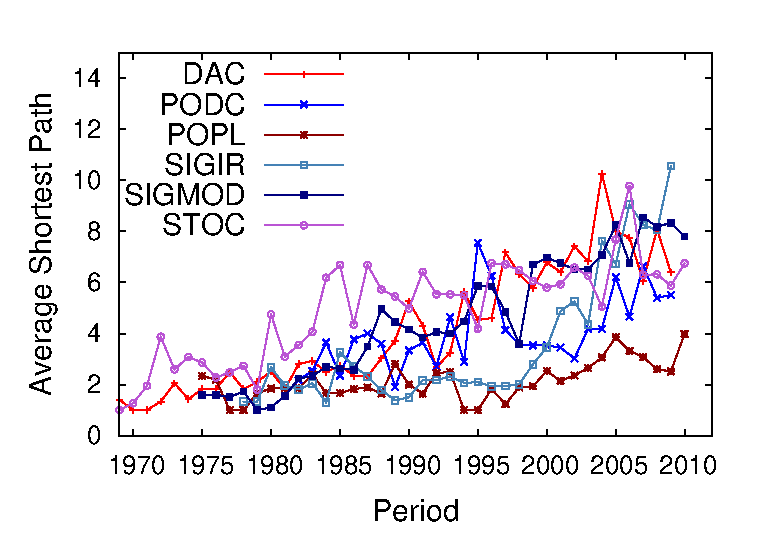
\includegraphics[scale=.33]{graficos/core_over_time/metricas_tradicionais/caminho_minimo_medio_slide_window_grupo_temporal_web.eps}
  }%
  \\
  \subfigure[Clustering coefficient]{%
    \label{fig:clustering_coefficient_slide_window}
    \includegraphics[scale=.33]{graficos/core_over_time/metricas_tradicionais/coeficiente_agrupamento_slide_window_grupo_temporal_web.eps}
  }%
  \subfigure[Largest connected component]{%
    \label{fig:largest_connected_component_slide_window}
    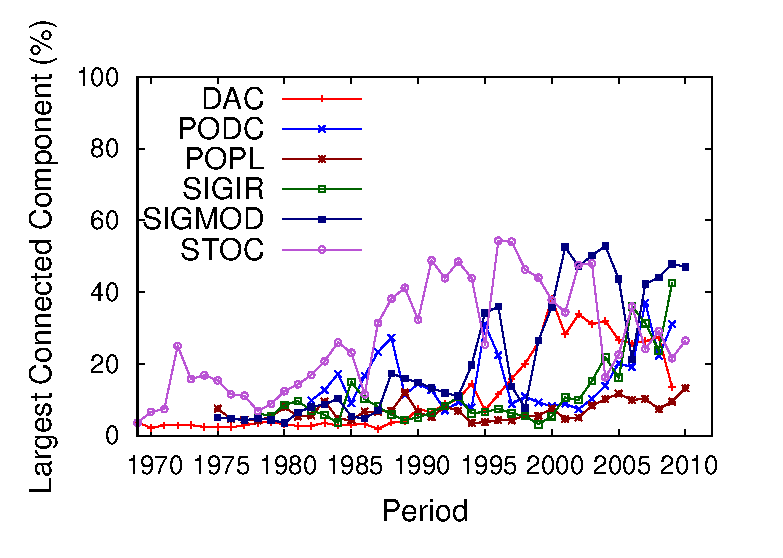
\includegraphics[scale=.33]{graficos/core_over_time/metricas_tradicionais/porcentagem_maior_componente_slide_window_grupo_temporal_web.eps}
  }%
  \\
  \subfigure[Average Degree]{%
    \label{fig:average_degree_slide_window}
    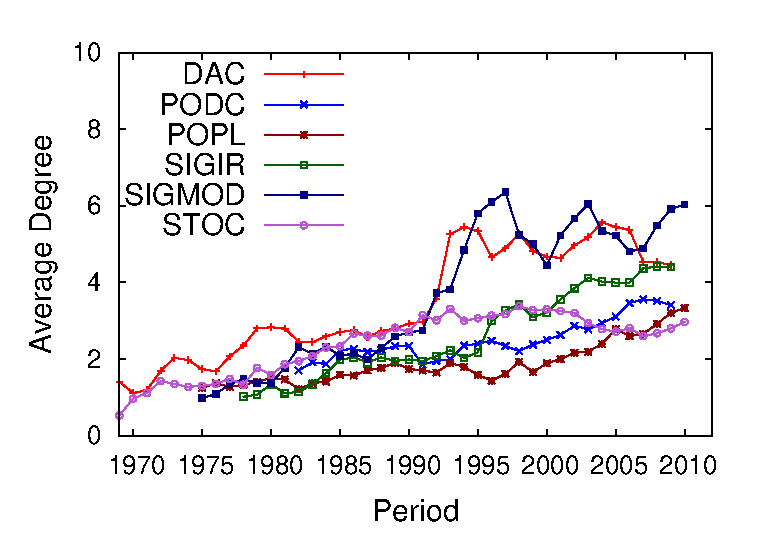
\includegraphics[scale=.33]{graficos/core_over_time/metricas_tradicionais/grau_medio_nodos_slide_window_grupo_temporal_web.eps}
  }%
  \end{center}
  \caption{Metrics using slide window of the 3 size}
  \label{fig:metrics_slide_window}
\end{figure}

In our studies about the core communities, we used the slide windows to understand how the core communities evolve. It is important
understand how the core community is clustered, because a core community very clustered may indicate a strong impact in the network.
The Figure \ref{fig:core_com_sigir_clustering_coefficient} and \ref{fig:core_com_sigmod_clustering_coefficient} shows the clustering 
coefficient of the SIGIR and SIGMOD, respectively. It is possible to see the behavior of the conference and the core community, the
two values are always so close, indicating that the core community has well clustering relative the conference.\\

\begin{figure*}[!htb]
  \begin{center}
  \subfigure[SIGIR - Clustering coefficient]{%
    \label{fig:core_com_sigir_clustering_coefficient}
    \includegraphics[scale=.33]{graficos/core_over_time/core_community/sigir_janela_3_core_coeficiente_agrupamento.eps}
  }%
  \subfigure[SIGIR - Average Degree]{%
    \label{fig:core_com_sigir_average_degree}
    \includegraphics[scale=.33]{graficos/core_over_time/core_community/sigir_janela_3_core_grau_medio_nodos.eps}
  }%
  \subfigure[SIGIR - Largest connected component]{%
    \label{fig:core_com_sigir_largest_connected_component}
    \includegraphics[scale=.33]{graficos/core_over_time/core_community/sigir_janela_3_core_maior_componente_conectado.eps}
  }%
  \\
  \subfigure[SIGMOD - Clustering coefficient]{%
    \label{fig:core_com_sigmod_clustering_coefficient}
    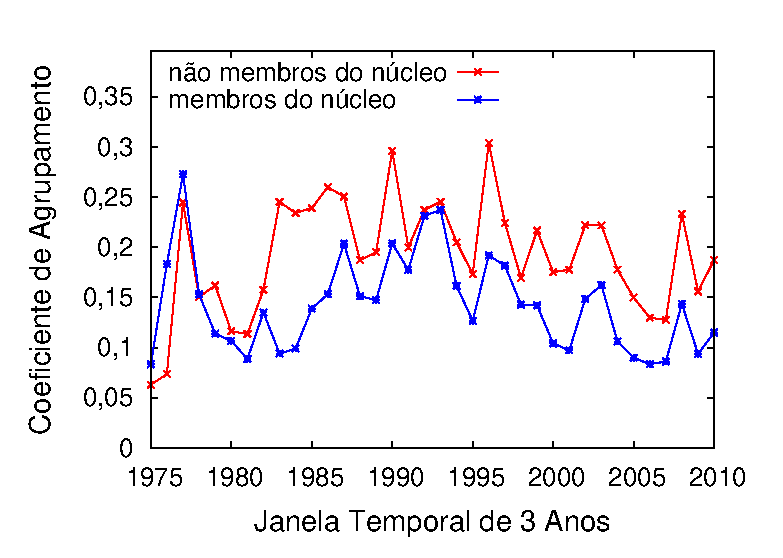
\includegraphics[scale=.33]{graficos/core_over_time/core_community/sigmod_janela_3_core_coeficiente_agrupamento.eps}
  }%
  \subfigure[SIGMOD - Average Degree]{%
    \label{fig:core_com_sigmod_average_degree}
    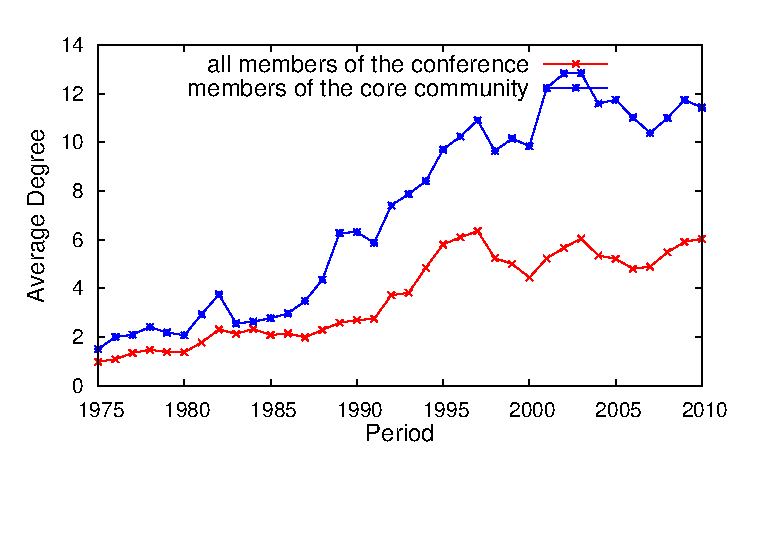
\includegraphics[scale=.33]{graficos/core_over_time/core_community/sigmod_janela_3_core_grau_medio_nodos.eps}
  }%
  \subfigure[SIGMOD - Largest connected component]{%
    \label{fig:core_com_sigmod_largest_connected_component}
    \includegraphics[scale=.33]{graficos/core_over_time/core_community/sigmod_janela_3_core_maior_componente_conectado.eps}
  }%
  \end{center}
  \caption{Metrics comparing the core community}
  \label{fig:metrics_comparing_core_community}
\end{figure*}

Over the years, a normal process is the researchers creates many links to another researchers, as students either or researchers of same 
institution or others physical places. The link to other researchers can be motivated by financial incetives the government, for exemple.
This scenario, the behavior of the links, can be seen in the Figure \ref{fig:core_com_sigir_average_degree} and 
\ref{fig:core_com_sigmod_average_degree}, it is important to note which this study do not use accumulated data, so the degree nodes of
the core community are always, generally, increasing over the years, reaching values higher than the community itself.\\
The core communities have the more important researchers in the network, in order, it is intuitive which many members of the core community
should be inside the largest connected component of the network, however, the Figure \ref{fig:core_com_sigir_largest_connected_component} and 
\ref{fig:core_com_sigmod_largest_connected_component} shows that this intuition is not totally correct, since in some periods the value of the
members of the core community into the largest connected component is 0.



\subsection{Average Community Core}

\begin{figure}[!htb]
\centering
\includegraphics[scale=.5]{graficos/average_core_score/average_core_score_slide_window_grupo_temporal_web.eps}
\caption{Average Core Score}
\label{fig:average_core_score}
\end{figure}

\subsection{Core communities and Network Structure}
{\bf reproduzir trabalho do rich club \cite{Xu:2010}}

We now examine to what extent the community core fluctuations affect the network structure.


\begin{table*}[!htb]
\centering
\caption{Corelation between average core score of the core community and the metrics of complex networks}
\label{tab:correlation_metrics}
{\small
\begin{tabular}{|l|c|c|c|c|c|c|c|} \hline
Conference & Diameter & Ave. Short P. & Clus. Coef. & Assort. & Larg. Com. Con. & Ave. Deg. Node & Num. Nodes\\ \hline
CCS & 0,34 & 0,2 & 0,23 & -0,2 & 0,45 & 0,14 & -0,13\\ \hline
CHI & 0,75 & 0,79 & -0,62 & -0,74 & 0,76 & 0,77 & 0,58\\ \hline
CIKM & 0,56 & 0,56 & -0,52 & -0,67 & 0,39 & 0,87 & 0,64\\ \hline
DAC & 0,8 & 0,85 & -0,49 & -0,63 & 0,76 & 0,92 & 0,84\\ \hline
HSCC & 0,17 & 0,45 & -0,62 & -0,71 & 0,87 & 0,55 & -0,55\\ \hline
ICSE & 0,81 & 0,83 & -0,52 & -0,84 & 0,68 & 0,8 & 0,78\\ \hline
ISCA & 0,63 & 0,55 & 0,54 & -0,32 & 0,63 & 0,81 & 0,41\\ \hline
ISSAC & 0,05 & 0,01 & -0,25 & -0,43 & -0,07 & 0,21 & 0,78\\ \hline
KDD & 0,1 & 0,17 & -0,33 & -0,67 & 0,2 & 0,14 & 0,2\\ \hline
MICRO & 0,35 & 0,35 & 0,28 & -0,36 & 0,52 & 0,51 & 0,36\\ \hline
MOBICOM & -0,04 & 0,11 & 0,13 & -0,65 & 0,23 & -0,09 & 0,02\\ \hline
Multimedia & 0,67 & 0,68 & -0,91 & -0,95 & 0,67 & 0,69 & 0,75\\ \hline
PODC & 0,4 & 0,42 & -0,23 & -0,2 & 0,13 & 0,68 & 0,57\\ \hline
POPL & 0,21 & 0,2 & 0,23 & -0,43 & 0,25 & 0,19 & 0,05\\ \hline
SAC & 0,48 & 0,59 & 0,16 & -0,39 & -0,55 & 0,16 & 0,23\\ \hline
SIGCOMM & 0,18 & 0,19 & 0,05 & -0,81 & 0,49 & 0,41 & -0,03\\ \hline
SIGCSE & 0,88 & 0,84 & -0,22 & -0,5 & 0,93 & 0,87 & 0,8\\ \hline
SIGDOC & 0,73 & 0,78 & -0,36 & -0,89 & 0,66 & 0,76 & 0,05\\ \hline
SIGGRAPH & 0,79 & 0,85 & -0,45 & -0,75 & 0,94 & 0,88 & 0,55\\ \hline
SIGIR & 0,83 & 0,85 & -0,42 & -0,77 & 0,7 & 0,89 & 0,88\\ \hline
SIGMETRICS & 0,31 & 0,24 & 0,3 & -0,44 & 0,37 & 0,64 & 0,43\\ \hline
SIGMOD & 0,78 & 0,81 & 0,27 & -0,61 & 0,77 & 0,87 & 0,68\\ \hline
SIGUCCS & 0,38 & -0,22 & 0,53 & -0,13 & 0,51 & 0,7 & 0,57\\ \hline
STOC & 0,61 & 0,63 & 0,54 & -0,37 & 0,82 & 0,88 & 0,68\\ \hline
{\bf Average} & {\bf 0,49} & {\bf 0,49} & {\bf -0,11} & {\bf -0,56} & {\bf 0,5} & {\bf 0,59} & {\bf 0,42}\\ \hline
\end{tabular}
}
\end{table*}





\section{Conclusions}

In this work we provide a deep investigation of the roles that members of the core of scientific communities play in the coauthorship network structure formation and evolution.
Our effort builds upon previous existent studies as it focuses on the core community instead of analyzing the evolutionary aspects of entire communities.  To do that, we define a
community core based on a metric namely \textit{core score}, an h-index derived measure that capture both, the prolifcness and involvement of authors in a community. Our analysis
suggests that the members of the core community work as bridges that connect smaller clustered research groups. Additionally, we note that the members of the core community tend to
increase the average degree of the network and decrease the assortativeness. More important, we note that variations on the members of the community core are strongly correlated
with variations on network properties.  Our study also highlights the importance to study the members of the community core and we hope that our observations might inspire future
community formation models.

As future work, we would like to extend and apply our analysis of the community core to other contexts such as massive multiplayer games and online social networks.







\bibliographystyle{abbrv}
\bibliography{short-references}  % sigproc.bib is the name of the Bibliography in this case
 
\end{document}
